\section{Problem Statement}
%We define the problem of path planning as follows: Given a start point and an end point, find the ``best'' path between them, where the definition of ``best'' depends on a set of preferences. Traditionally, the selected path will depend on two things: the location of obstacles and the length of the path, i.e. the planned paths are generally the shortest path to the goal that avoids collisions with any other objects. Finding such a path is generally easy. However, beyond avoiding collisions and getting to the destination efficiently, there are a number of other factors that can factor into which path is considered ``best.'' 

We define the problem of path planning with non-lethal constraints as follows: find a path from a starting location to a goal while not colliding with any obstacles and maximizing the distance from the path to a set of non-lethal obstacles while minimizing the overall length of the path. The duality of maximizing the one quantity while minimizing the other results in a continuum of different paths that could be considered optimal depending on the weighting of the two sides. 

\begin{figure}
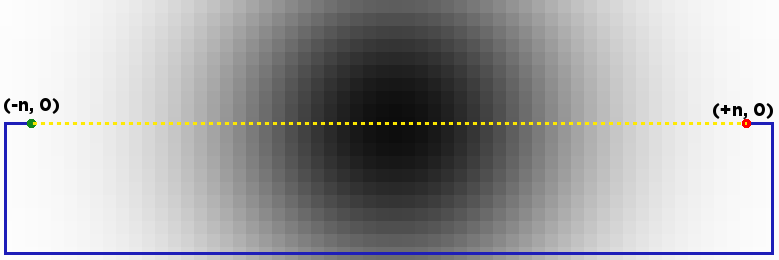
\includegraphics[width=\columnwidth]{graphix/TwoPaths.png}
\caption{Two Simple Paths - The dotted yellow path is the shortest possible path. The solid blue path is the path with the lowest possible cost (within the bounds of the costmap). The tint of each cell is proportional to its cost. The green and red dots indicate the start and goal points respectively. }
\label{fig:twopaths}
\end{figure}

If we prioritize the shortest possible path (as most planners do), we end up with the straight path seen in Figure \ref{fig:twopaths}, which does not make any attempt to avoid the obstacle. (Note that there are no lethal obstacles shown in the figure.) However, the lowest cost regions are along the border of the costmap, so if lowest cost becomes the priority, a longer more round-about path will be taken. 

A more formal statement of the problem includes the following elements. First, a grid of discretized cells lying in a two dimensional plane, denoted by $x$ and $y$. Each cell has a non-negative cost, denoted by $C(x,y)$, where all cells with $C(x,y)\ge L$ are considered to be lethal, and the rest are non-lethal.  Given starting and goal cells (from the non-lethal subset), find a path from one to the other that moves from one to the other moving through only non-lethal cells that minimizes the length and total cost. 

In the case of a 4-connected grid, one efficient way of calculating such a path is

\[ \min_{\forall \mathrm{path} p} \Phi(p) = \min_{\forall \mathrm{path} p} \sum\limits_{(x,y) \in p}^{} \Big[ C(x,y) + P \Big] \]

where $\Phi(p)$ represents the combination of the path length and summation of $C(x,y)$, and $P$ is the path constant. That is to say, in addition to minimizing the total cost, we minimize the total cost plus some constant value for each cell entered. The value of $P$ is our primary means of controlling how much path length is considered vs. total cost. If $P=0$, then the long path in Figure \ref{fig:twopaths} will be planned, and if $P$ is rather large, the short straight path will be taken. 


For our initial pass analyzing these paths, we are going to assume for simplicity a 4-connected grid rather than an 8 or more connected grid, since such paths would involve scaling the costs and path constant proportionally to how long the path is in each cell. 

For purposes of this paper, let us further refine the problem to reduce the number of cases we must consider. First, let us consider paths that go from $(-n, 0)$ to $(n, 0)$. This means that the costmap will be aligned to the primary direction of travel (i.e. the shortest path passes through $2n$ cells. When these are unaligned, the paths can be substantially different in shape, and will require analysis beyond the scope of this paper, as we describe in the Future Work section. We further assume that there are no lethal cells in our costmap, since path planning algorithms already do a fine job of avoiding lethal obstacles, so for now, we can presume that any non-lethal plan is a repeated application of planning with only non-lethal obstacles. Along the same lines, we define $C(x,y)$ to be the cost as though there were a non-lethal obstacle at $(0,0)$, where the cost of approaching such an obstacle is $f(x,y)$ for some function $f$. 

In the following sections, we will see how different selections for $f$ and how $f$ is parameterized can have vastly different effects on the path. 
